%
% File acl2015.tex
%
% Contact: car@ir.hit.edu.cn, gdzhou@suda.edu.cn
%%
%% Based on the style files for ACL-2014, which were, in turn,
%% Based on the style files for ACL-2013, which were, in turn,
%% Based on the style files for ACL-2012, which were, in turn,
%% based on the style files for ACL-2011, which were, in turn, 
%% based on the style files for ACL-2010, which were, in turn, 
%% based on the style files for ACL-IJCNLP-2009, which were, in turn,
%% based on the style files for EACL-2009 and IJCNLP-2008...

%% Based on the style files for EACL 2006 by 
%%e.agirre@ehu.es or Sergi.Balari@uab.es
%% and that of ACL 08 by Joakim Nivre and Noah Smith

\documentclass[11pt]{article}
\usepackage{acl2015}
\usepackage{times}
\usepackage{url}
\usepackage{latexsym}
\usepackage{graphicx}
\usepackage{listings}
\usepackage{multicol}
\usepackage{xcolor}

\lstset{
    basicstyle=\ttfamily\footnotesize,
    keywordstyle=\bfseries\color{black},
    commentstyle=\itshape\color{gray},
    breaklines=true,
    columns=fullflexible
    frame=single
}

%\setlength\titlebox{5cm}

% You can expand the titlebox if you need extra space
% to show all the authors. Please do not make the titlebox
% smaller than 5cm (the original size); we will check this
% in the camera-ready version and ask you to change it back.


\title{ScamGuard: Enhancing Online Safety with Scam Detection and LLM-based Explanation Insights}

\author{A. Shahnawaz, A. Zahid, D. K. Khan, M. S. Abbas, N. Hakim, and Ubaid \\
  Lahore University of Management Sciences
\\
  {\tt \{23030024, 25100247, 24100139, 20030038, 24100131, 23030027\}@lums.edu.pk} \\
}
\date{}

\begin{document}
\maketitle
\begin{abstract}
    ScamGuard is a comprehensive solution for detecting online scams and providing insightful explanations. Our system integrates multiple large language models (LLMs) to identify potential scams in text or audio inputs, making it accessible to diverse users, including those who only know Urdu. By leveraging Streamlit for integration of speech-to-text module, LLMs, and a minimal interface, ScamGuard provides consolidated predictions and detailed explanations for why a text might be scam. The system's primary components include six LLMs, 6 for scam predictions and one for consoldiation of results from all LLMs, a Whisper-based ASR module, and an intuitive web-based interface. All LLMs showed similar performance on English but Gemini and GPT excelled in Urdu as well, therefore we switched between the two as consolidators. Testing showed impressive performance both in English and Arabic Script Urdu.
\end{abstract}

\section{Implementation details}
\subsection{System Design}

Our system design involved the following steps: 1) Stacking multiple LLMs for scam detection, 2) Adding a speech-to-text module to allow audio input, and 3) Integration of LLMs and ASR with Streamlit and designing the user interface.

{\textbf{\textit{Scam Detection and Explanation}}}

With the goal of facilitating easier scam detection, we developed ScamGuard, a solution that processes user input to classify whether it indicates a scam or not. To make it more accessible to the Pakistani population and individuals with limited literacy, we included an audio feature where users can provide an audio description or a recording of the potential scam.

We leveraged Streamlit to seamlessly integrate our Automatic Speech Recognition(ASR), Large Language Models(LLMs), and User Interface(UI). We chose Streamlit for its rapid prototyping capabilities, smooth integration with existing machine learning pipelines, and a clean user interface. For these reasons, we were able to launch a fully functional, ML-powered web application on a local host.

The output of ScamGuard includes individual predictions from each LLM on whether the text or audio input is a scam, a consolidated probability score derived from the outputs of all LLMs, and a detailed explanation outlining the reasons why the input might be considered a scam.

{\textbf{\textit{Speech-to-text Module }}}

Our LLM module requires text as input for scam classification. To handle audio input, we convert it to text as a preprocessing step using the Whisper-base model. Whisper \cite{radford2022robust}, a Transformer-based encoder-decoder model, or sequence-to-sequence model, is trained on 680k hours of labeled speech data using large-scale weak supervision. The models are trained on either English-only or multilingual data and are available in five configurations of varying sizes. We chose Whisper-base (74M parameters), a multilingual model, to cater to audio input in both Urdu and English. This ensures that our application can effectively classify scams from Urdu audio inputs.

We tested the performance of whisper-base model with various English and Urdu input audios and it demonstrated remarkable generalization across diverse domains without requiring fine-tuning, which is why we opted not to fine-tune it for our application. The model's performance only deteriorated when background noise was excessive and overshadowed the primary audio. Consequently, this limitation implies that our application requires audio input with moderate noise levels for optimal performance.

{\textbf{\textit{LLMs Component }}}

For performance evaluation and selection of large language models (LLMs), we consulted the literature. \cite{koide2024chatspamdetector} analyzed four models: GPT-3.5-Turbo, GPT-4, Llama2-70B, and Gemini Pro, all achieving over 95\% accuracy in spam detection. Similarly, \cite{patel2024largelanguagemodels} assessed various LLMs, including GPT-4, GPT-3.5, Llama2, and Mistral-7B, on a subset of Kaggle's fraudulent email corpus. Consistently across studies, the GPT models performed exceptionally well in identifying spam, scam, and phishing attempts. The decoder-only design  allows these models to effectively comprehend natural language flow enabling the identification of inconsistencies that hint at phishing and potential fraudulent scenarios.


Using both literature and our own testing, we selected seven LLMs:

\begin{enumerate}
    \item \textbf{Mistral 8x22B} is open-source, with 64K tokens context windo.  It is a sparse Mixture-of-Experts (SMoE) model, and activates only 39 billion of its 141 billion parameters, providing exceptional cost efficiency.
    
    \item \textbf{Llama 3-70B} is an open-source auto-regressive language model with an optimized transformer architecture, pre-trained on over 15 trillion tokens sourced from publicly available data. It is fine-tuned with instruction datasets and 10 million human-annotated examples.
    
    \item \textbf{Phi-2} is an open-source, 2.7 billion-parameter Transformer trained with data sources from Phi-1.5, augmented by synthetic NLP texts and carefully filtered websites. Phi-2 demonstrates near state-of-the-art performance among models with fewer than 13 billion parameters, excelling in common sense, language understanding, and logical reasoning.
    
    \item \textbf{StripedHyena-Nous-7B} is the first alternative model that can compete with the top open-source Transformers in both short- and long-context tasks. It matches or outperforms models like Llama-2 and Mistral 7B on OpenLLM leaderboard tasks, particularly excelling in long-context summarization. It employs grafting techniques to incorporate the best components of Transformers and Hyena architectures.
    
    \item \textbf{OLMo-7B-instruct} is open-source and leverages the Allen AI's Dolma dataset, which contains a 3 trillion token open corpus for model pre-training. With four 7B variants trained to at least 2 trillion tokens each, this model provides extensive checkpoints, inference code, and evaluation metrics.
    
    \item \textbf{Gemma-7B} is a family of lightweight, open models built on the research used for Google's Gemini models. These decoder-only, text-to-text models are adept at tasks like question answering, summarization, and reasoning. Despite their smaller size, they are versatile and efficient enough to run on laptops or local cloud infrastructure. They are trained on 6 trillion tokens from diverse text sources.

    \item \textbf{GPT-3.5-Turbo} is an optimized variant of OpenAI's GPT-3 model family. It supports a wide range of tasks such as summarization, translation, and conversational understanding, while offering flexible deployment options. This model has been instrumental in providing high-quality answers across numerous domains due to its ability to capture and predict contextual language patterns effectively, as evident in literature.

    \item \textbf{Gemini-1.0} is a state-of-the-art LLM developed by Google. These model is known for its versatility and efficiency in tasks such as question answering, summarization, and reasoning. Built with a decoder-only architecture and trained on a vast corpus of high-quality, diverse text, Gemini model is optimized for natural language understanding and generation. Its provide good performance across multiple languages and topics, making it suitable for a wide range of applications.
    
\end{enumerate}

The input text is passed through each of the six LLMs, generating predictions and explanations. These outputs are then passed to GPT-3.5(or Gemini), which serves as a consolidator, merging the predictions and providing with a explanation for why a text might be a scam.

Initially, GPT-3.5 was used as the final LLM in our system, consolidating the outputs of all other models. However, we ran out of tokens during testing and evaluation, and switched to Gemini to perform this role. Figure \ref{fig:flowchart} illustrates the current system design, which excludes GPT-3.5, although it was originally included and demonstrated superior performance. In the final system design, we have 6 predictor LLMs and one consolidator LLM.



\begin{figure*}[ht]
    \centering
    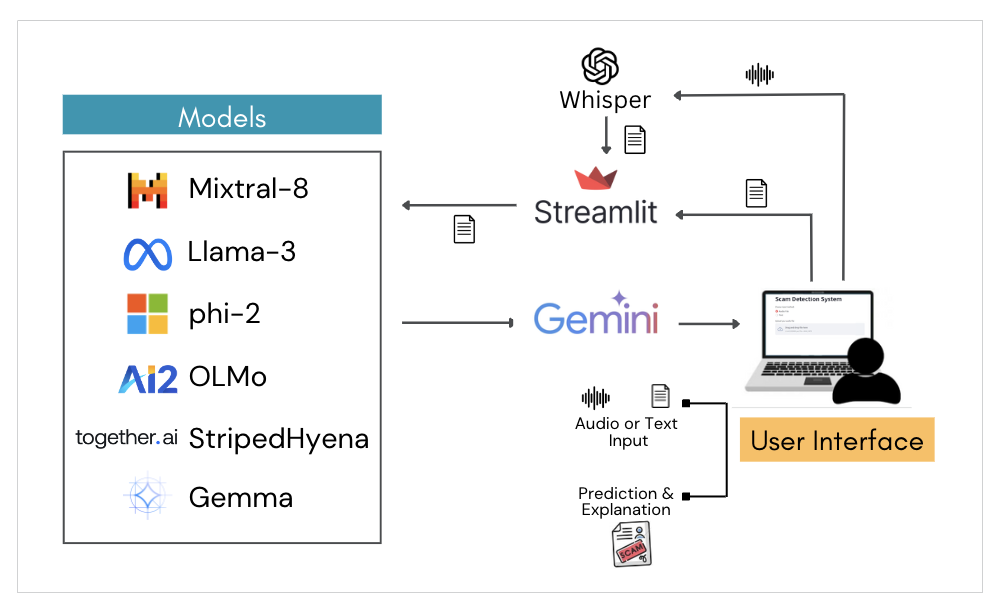
\includegraphics[width=0.8\textwidth]{flowchart.png} % Replace 'example.png' with your image filename
    \caption{Overview of ScamGuard's System Design, application's component interactions and data flow}
    \label{fig:flowchart}
\end{figure*}


\section{Deployment}
The app repository is hosted on GitHub, containing the Streamlit app. To run the app, first pull the repository.
Ensure that Streamlit and Whisper are installed before executing this command. You can install Streamlit with:
\begin{lstlisting}[language=bash]
pip install streamlit
\end{lstlisting}
For Whisper, use:
\begin{lstlisting}[language=bash]
pip install git+https://github.com/openai/whisper.git
\end{lstlisting}
To install everything at once, you can run requiremnets.txt.

You'll also need to run the following command in windows powershell to install chocolatey that will then, set up the ffmpeg for whisper:

\begin{lstlisting}[language=bash]
Set-ExecutionPolicy Bypass -Scope Process -Force; 
[System.Net.ServicePointManager]::SecurityProtocol = 
[System.Net.ServicePointManager]::SecurityProtocol -bor 3072; 
iex ((New-Object System.Net.WebClient).DownloadString('https://chocolatey.org/install.ps1'))
\end{lstlisting}

Next, install ffmpeg via Chocolatey:
\begin{lstlisting}[language=bash]
choco install ffmpeg
\end{lstlisting}
This setup will ensure you have everything required to run the app.
Now, navigate to the appropriate directory, and use the command:
\begin{lstlisting}[language=bash]
streamlit run ScamGuard-main/View/app.py
\end{lstlisting}
This command will start app for you in the browser. 

The app is hosted locally, allowing the user to interact with it through a web browser. After following the setup instructions and running the app, you can access it by opening a web browser and navigating to the appropriate local address, typically http://localhost:8501. The browser will provide interface for interacting with the Streamlit application.
The idea behind using browser as interface was to provide users with a simple and uncomplicated way to interact with the app. Streamlit allowed for rapid prototyping capabilities and smooth integration with existing machine learning pipelines. We plan to dockerize our Streamlit app and host it on Google Cloud(Thanks to their \$300 free credit offer). 

\section{Experiments and Iterations}

To improve , we employed a systematic, iterative approach. First, we tested LLM individually using various prompts, to get insights into their respective strengths and weaknesses, particularly with Urdu language. By analyzing their responses to different prompts, we identified areas where performance lacked and where they excelled. This detailed analysis allowed us to refine a specialized prompt template tailored specifically for the consolidator LLM(GPT) which is shown in Figure 2. This template became the standard by which the consolidator LLM would interpret and analyze the text input and outputs of individual LLMs. Our refinements include clarifying instructions and emphasizing key aspects such as identifying impersonation and social engineering tactics.
We later switched to using Gemini for the consolidation process. In doing so, we refined the prompt initially created for GPT by incorporating additional details. This prompt not only includes the predicted probability of each input being a scam, but also gathers and presents the individual predictions and total probability of scam. By providing this level of granular information, the updated prompt enables Gemini to assess and interpret the results from all contributing models, producing a more detailed explanation for the classification. This approach provides more comprehensive insights to the user.

\begin{figure*}[ht]
    \centering
    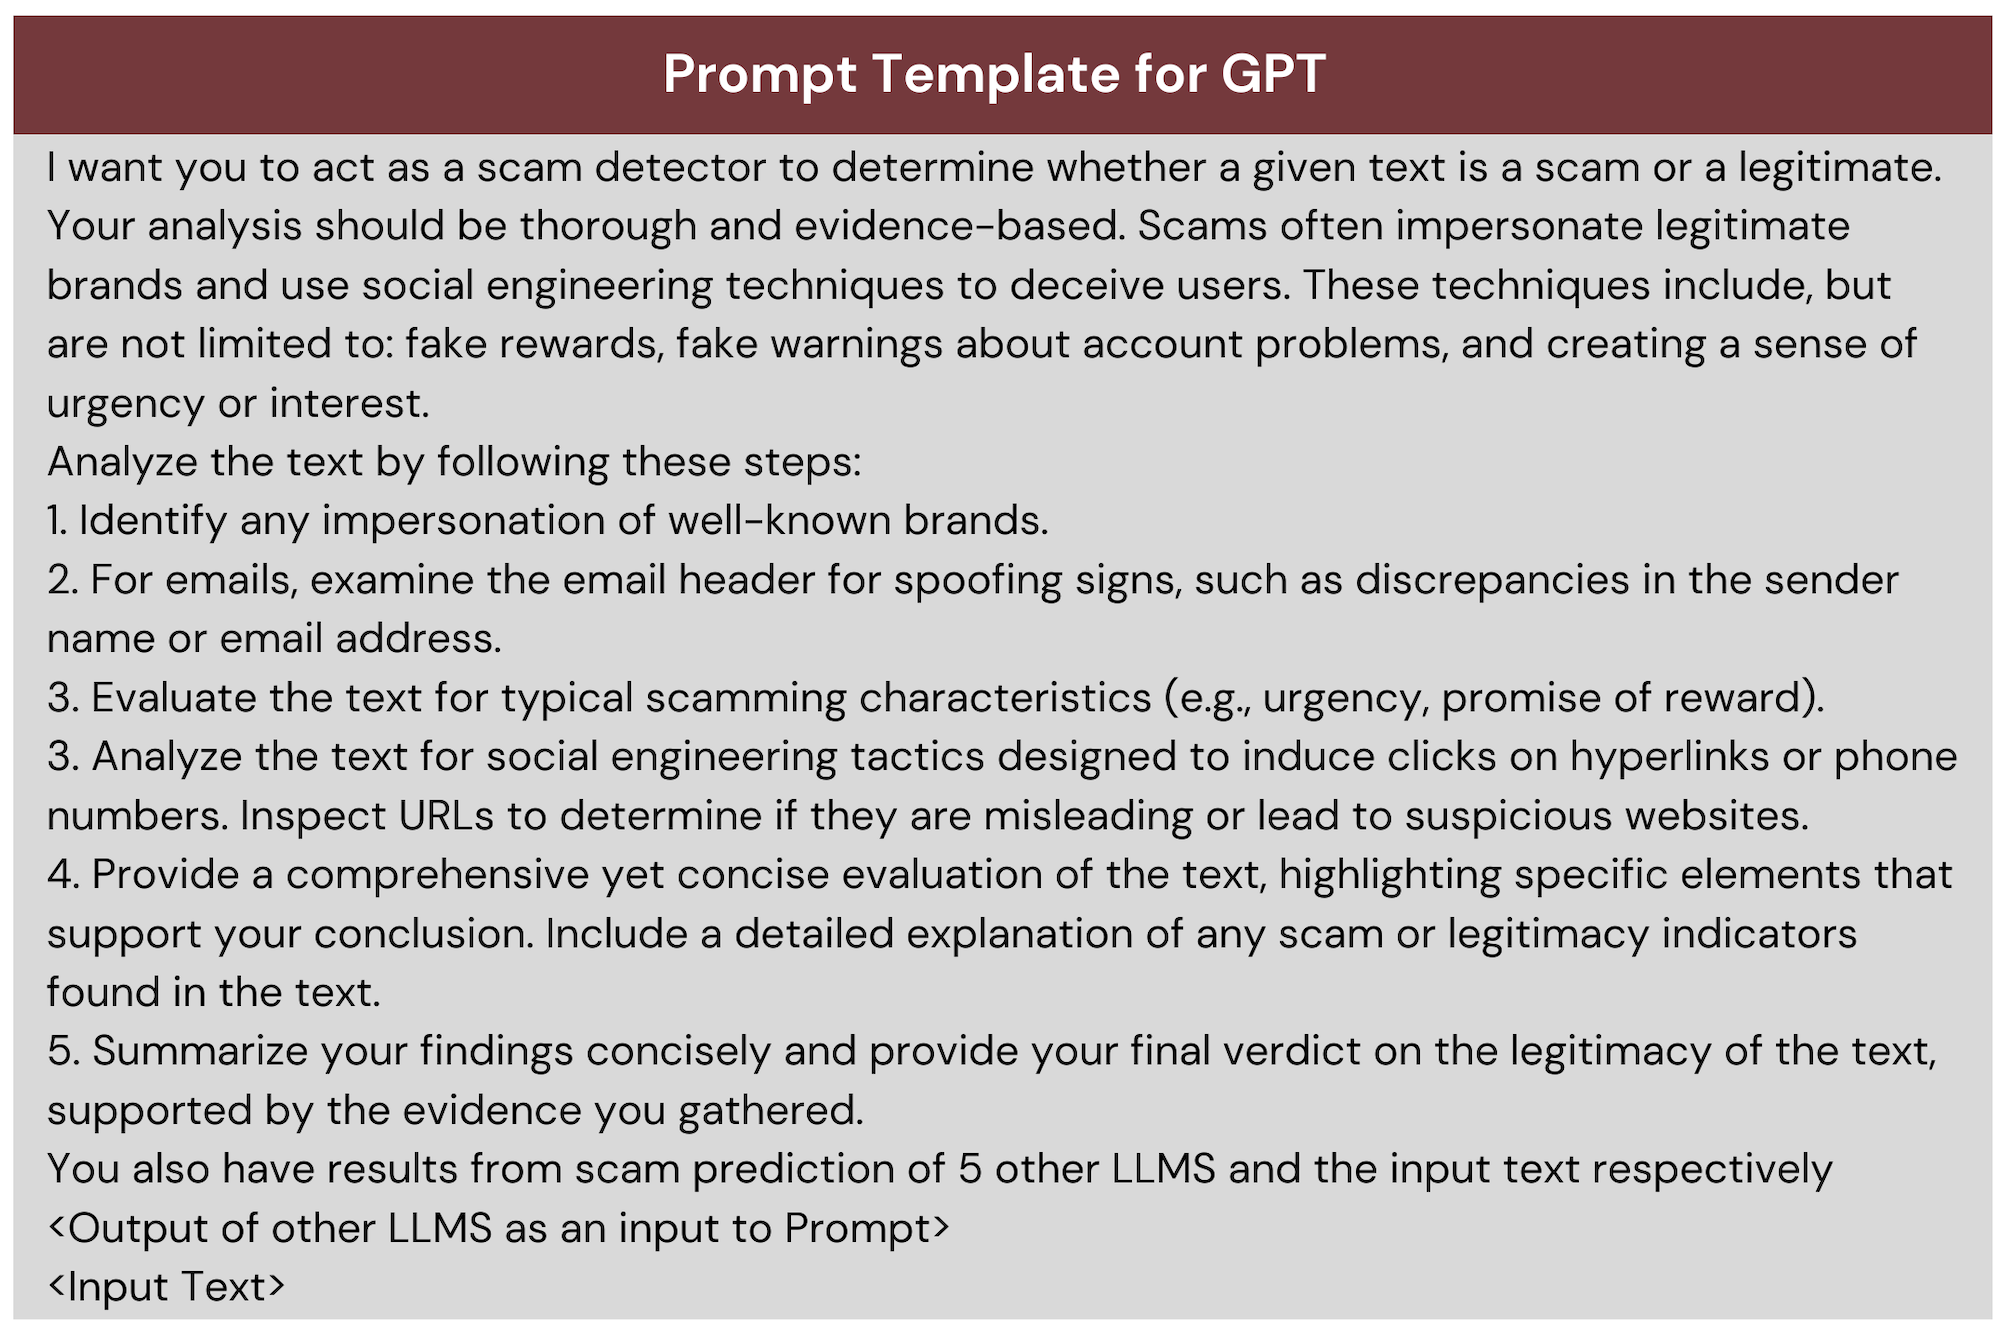
\includegraphics[scale=0.5]{prompt.png} 
    \caption{Prompt Template for GPT as consolidator LLM}
    \label{fig:prompt}
\end{figure*}

\begin{figure*}[ht]
    \centering
    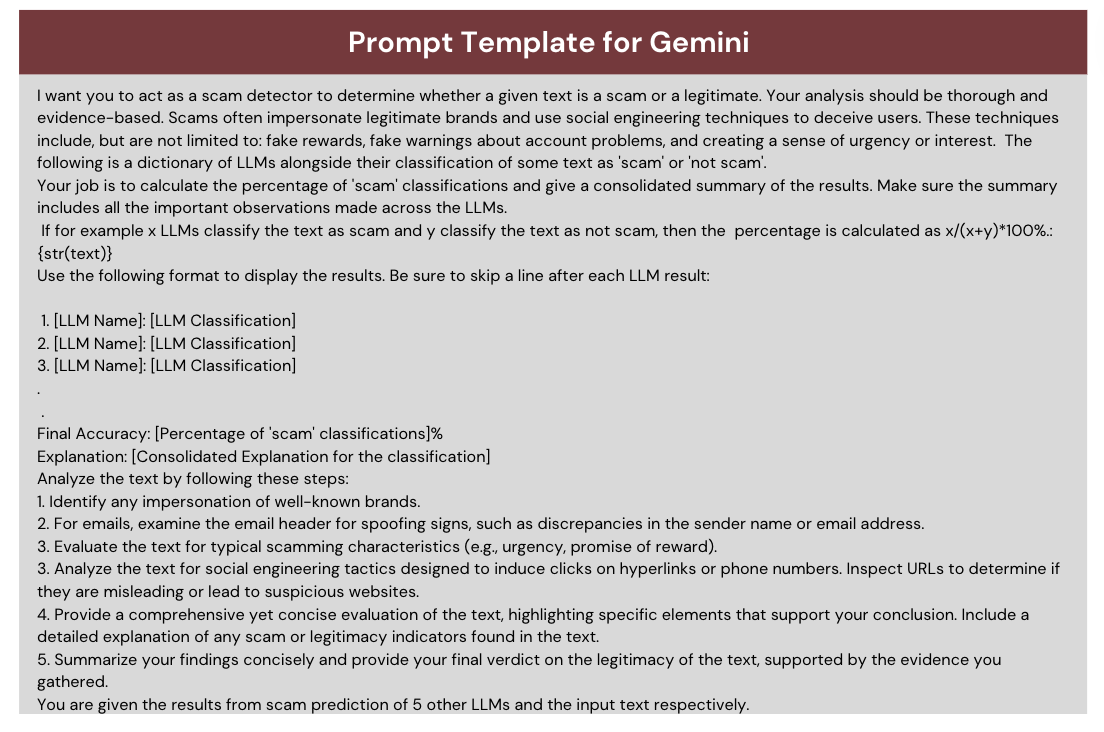
\includegraphics[scale=0.75]{gemini_prompt.png} 
    \caption{Prompt Template for Gemini as consolidator LLM}
    \label{fig:gemini_prompt}
\end{figure*}

\begin{figure*}[ht]
    \centering
    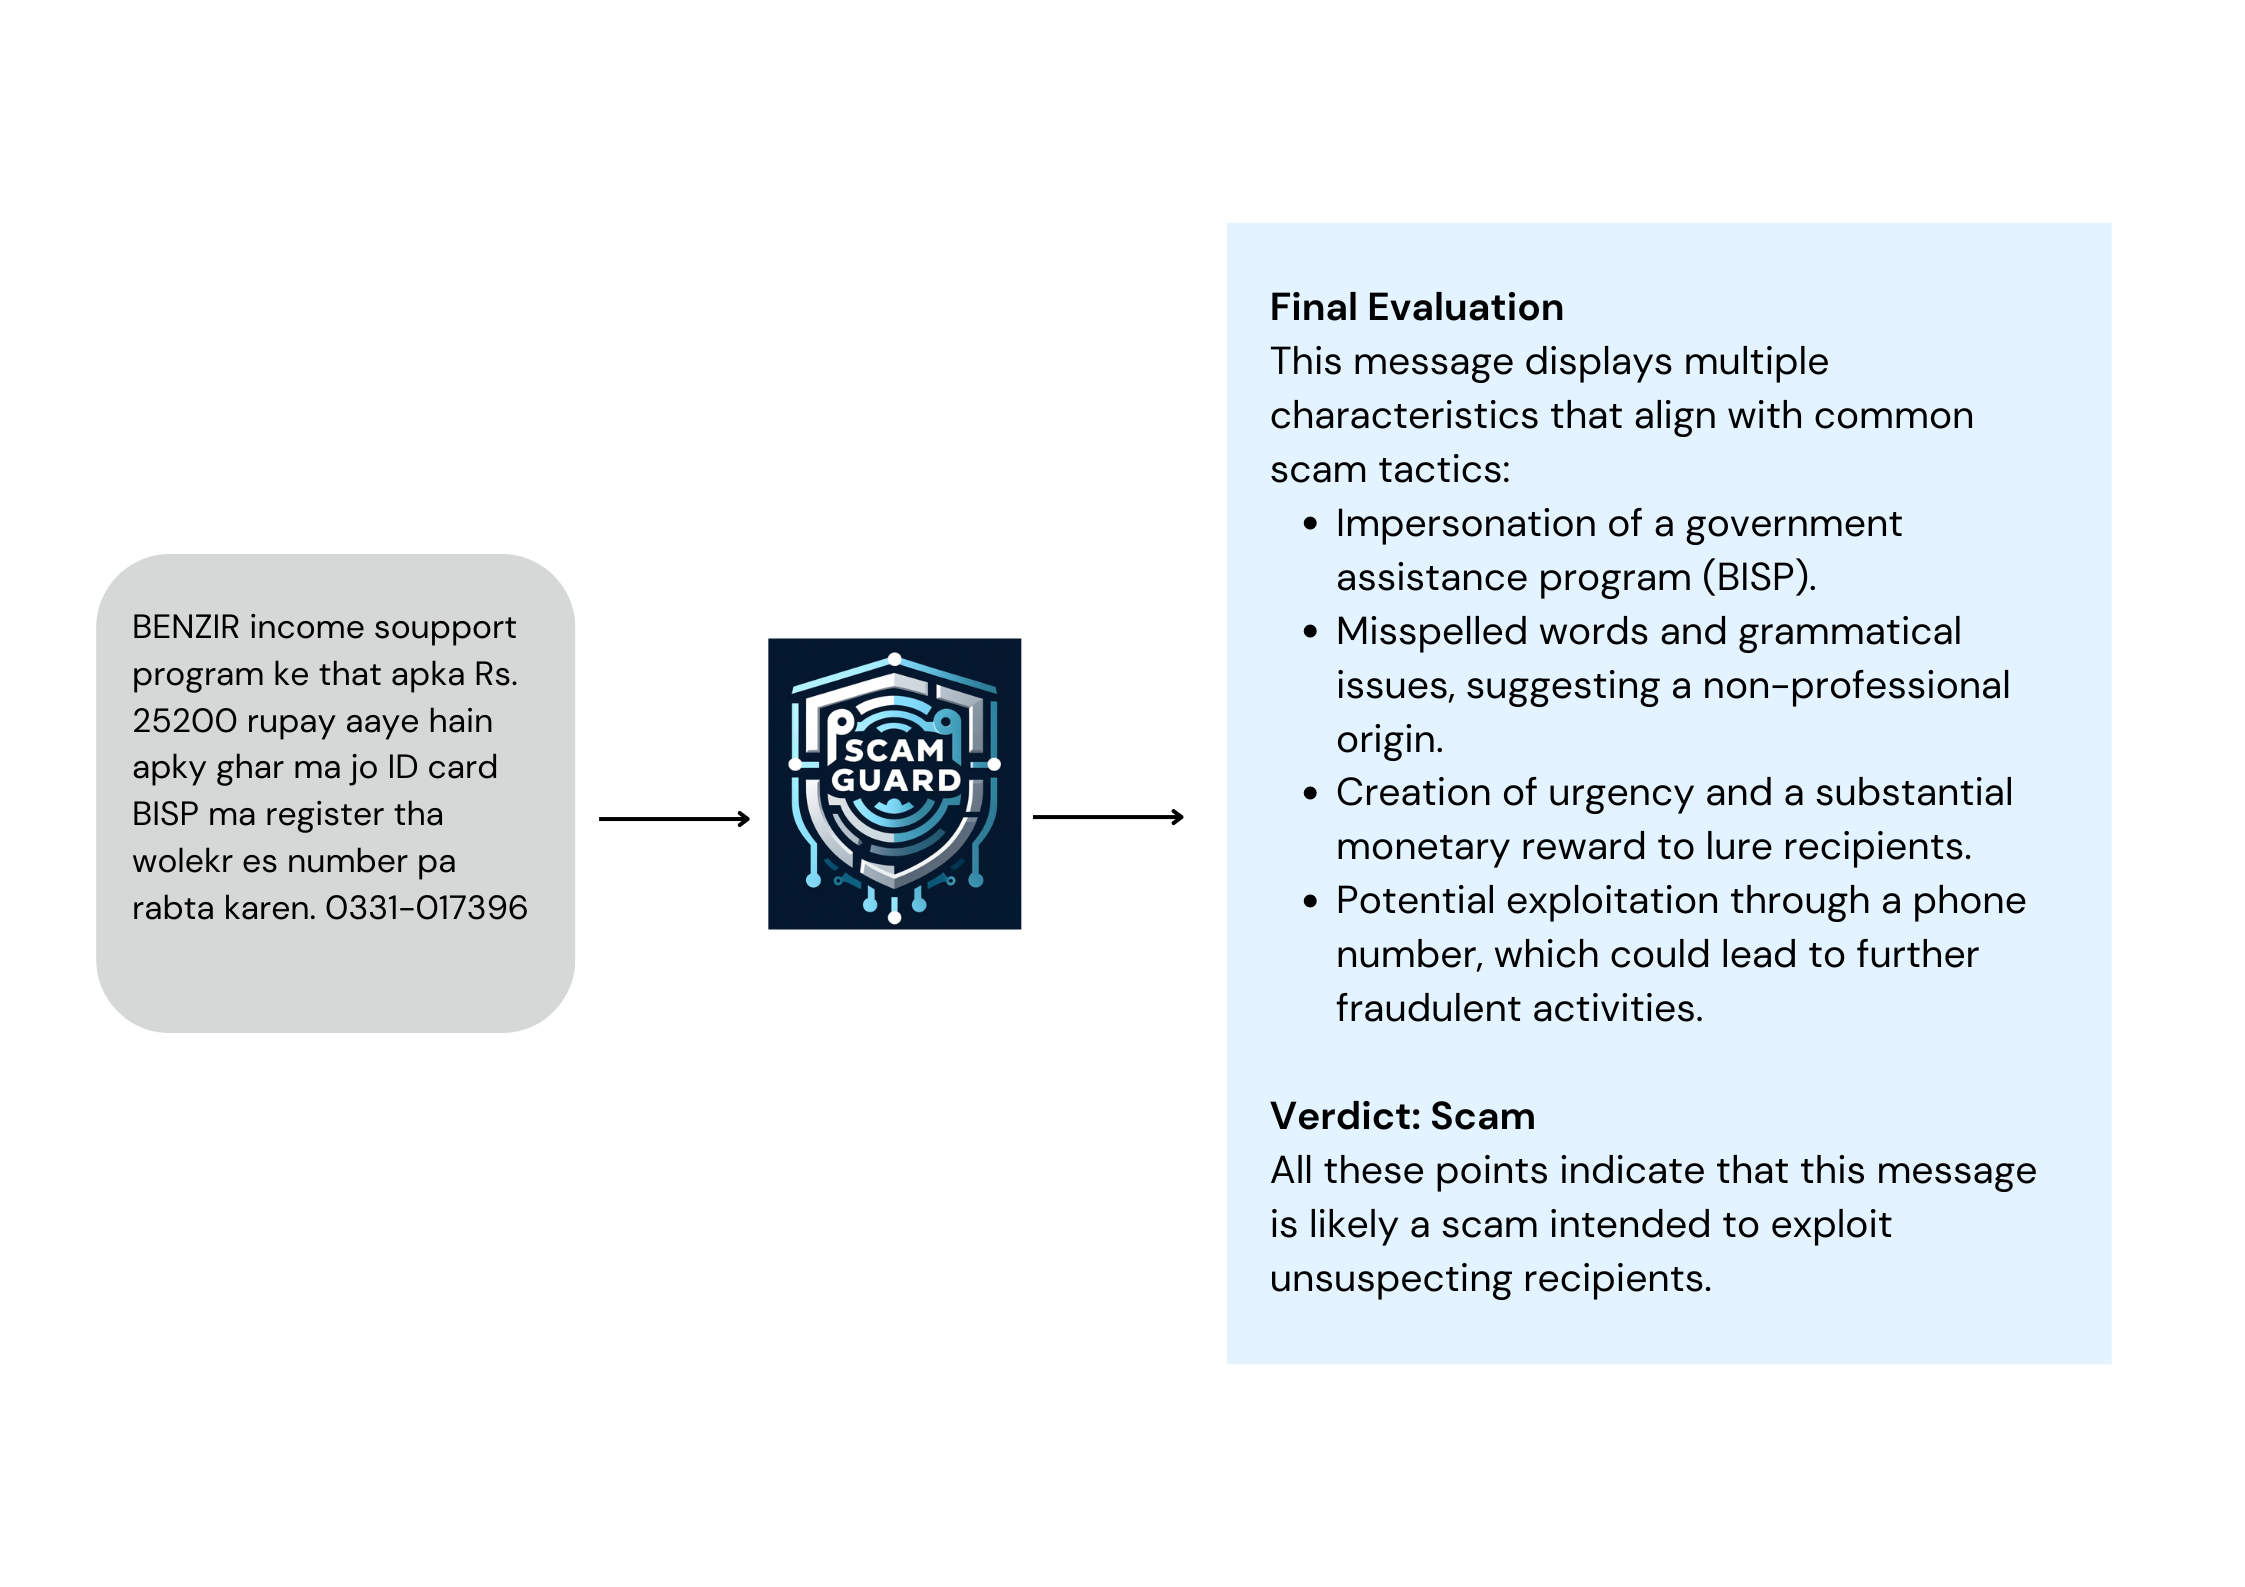
\includegraphics[scale=0.2]{gpt.png} 
    \caption{Scam detection using GPT consolidator LLM with English Explanation}
    \label{fig:gpt}
\end{figure*}
\begin{figure*}[ht]
    \centering
    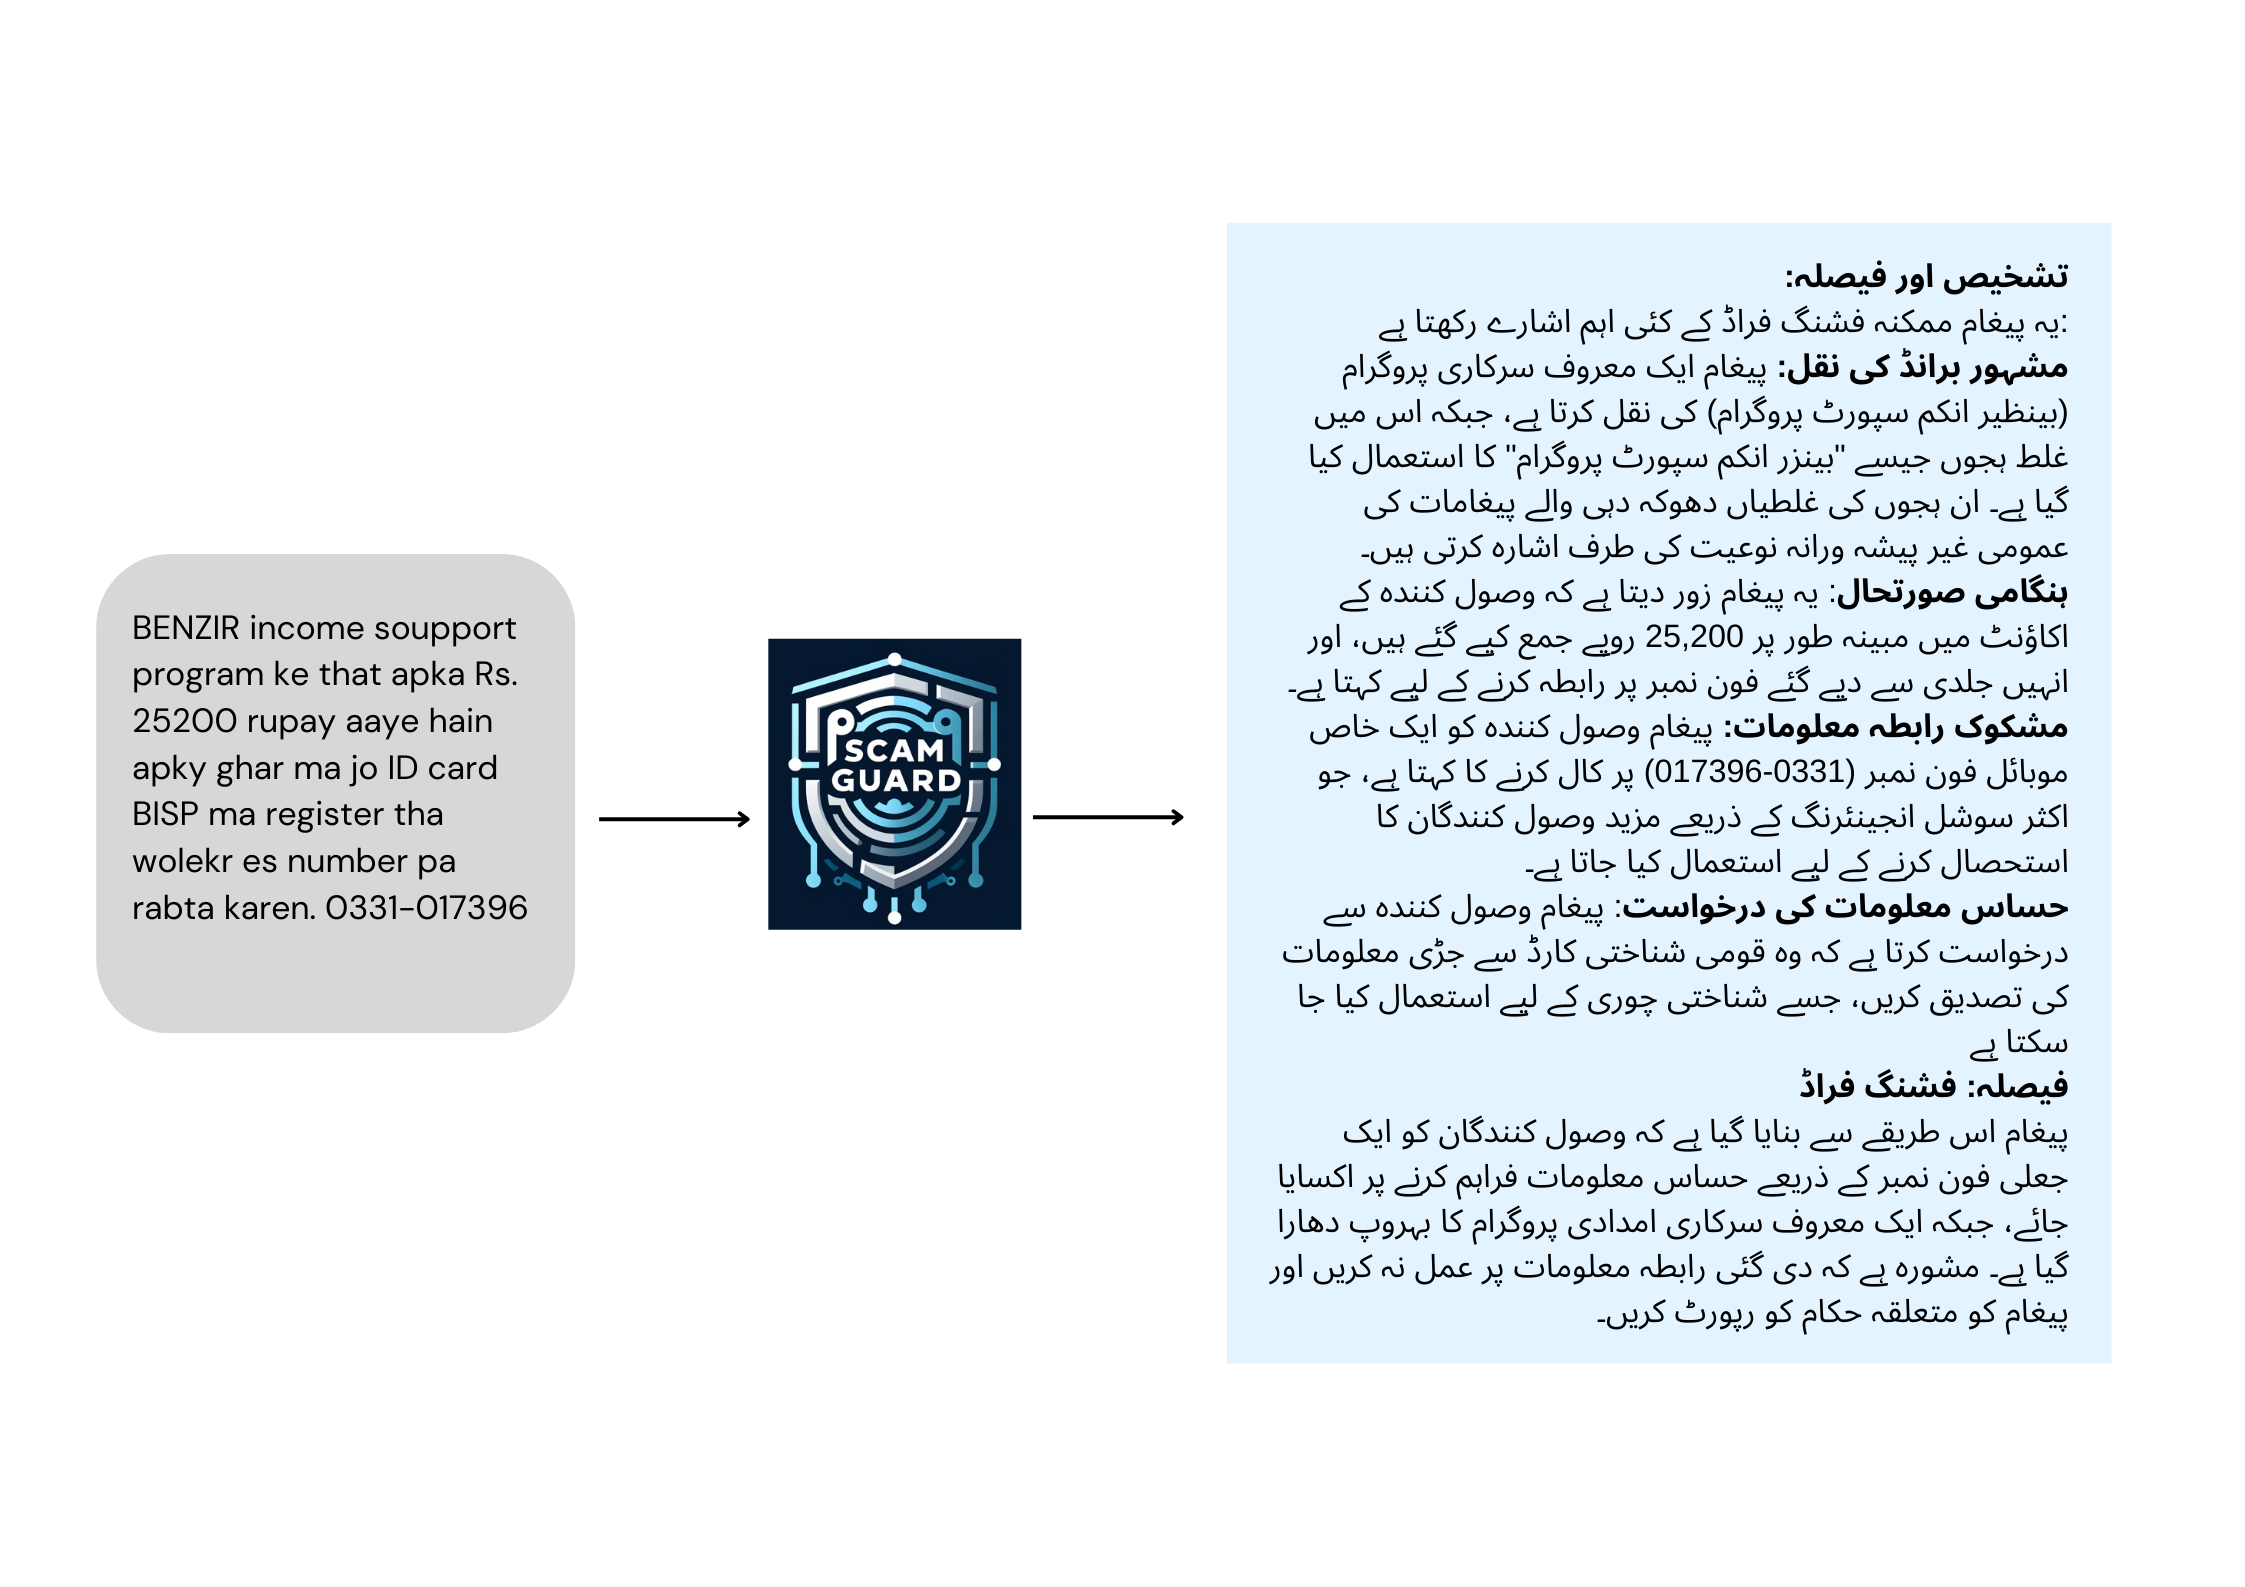
\includegraphics[width=0.8\textwidth]{gpt_urdu.png} 
    \caption{Scam detection using GPT consolidator LLM with Urdu Explanation}
    \label{fig:gpt_urdu}
\end{figure*}

\begin{figure*}[ht]
    \centering
    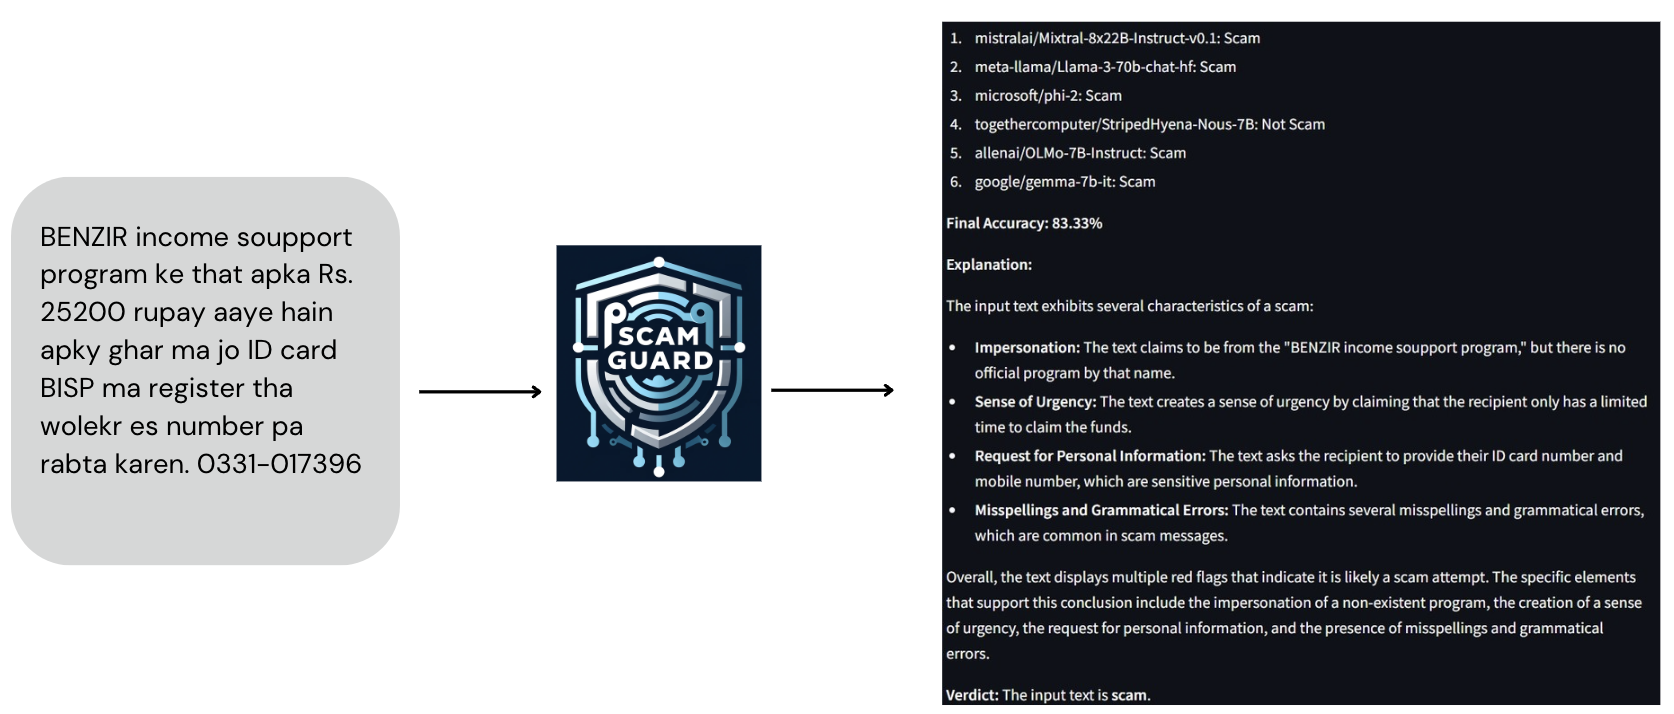
\includegraphics[width=0.8\textwidth]{gemini.png} 
    \caption{Scam detection using Gemini consolidator LLM}
    \label{fig:gemini}
\end{figure*}

Figures \ref{fig:gpt} and \ref{fig:gemini}  demonstrate sample outputs generated by both GPT and Gemini as consolidators. The results reveal that GPT consistently produced more cohesive responses when dealing with Urdu scam messages. This cohesiveness ensured that scam indicators were accurately identified and explained in a structured manner, enabling comprehensive evaluations.

\section{Reflections}

{\textbf{\textit{{What worked well?}}} Initially, we intended to use a separate machine learning model to classify text and then have an LLM provide explanations, as outlined in our project proposal. However, after experimenting with several LLMs, we found that their scam detection surpassed that of our classifier. As a result, we used LLMs for both classification and explanation. Among the options tested, GPT and Gemini worked best for Urdu, but GPT delivered the strongest overall performance.

{\textbf{\textit{{What didn’t work well?}}} Our GPT credits ran out on the final day, so we had to use Gemini for consolidation. While it performed adequately compared to GPT, it didn't fully match up. Additionally, many LLMs struggled to identify Urdu scams, likely due to limited support for the language. We also attempted to dockerize the Streamlit app and host it on Google Cloud, but couldn't complete it within the project timeline.

{\textbf{\textit{What would be the next step to improving your system?}}} A valuable next step would be to gather a comprehensive dataset of scams over time and fine-tune a model using this data. We aim to deploy it in the cloud to see if it can effectively help the general population recognize scam tactics and educate themselves on common indicators.

{\textbf{\textit{How could you have remedied what went wrong?}} Overall, nothing major went wrong—just minor issues like prompt misfires and some trial-and-error with API integration. The primary challenge was running out of tokens, which could have been mitigated by not being broke.

\section{Demonstration}
Figures \ref{fig:demo} shows the main landing page of the application and outputs for text and audio. \ref{fig:gemini} shows the output of system with the final prompt. 

\begin{figure*}[ht]
    \centering
    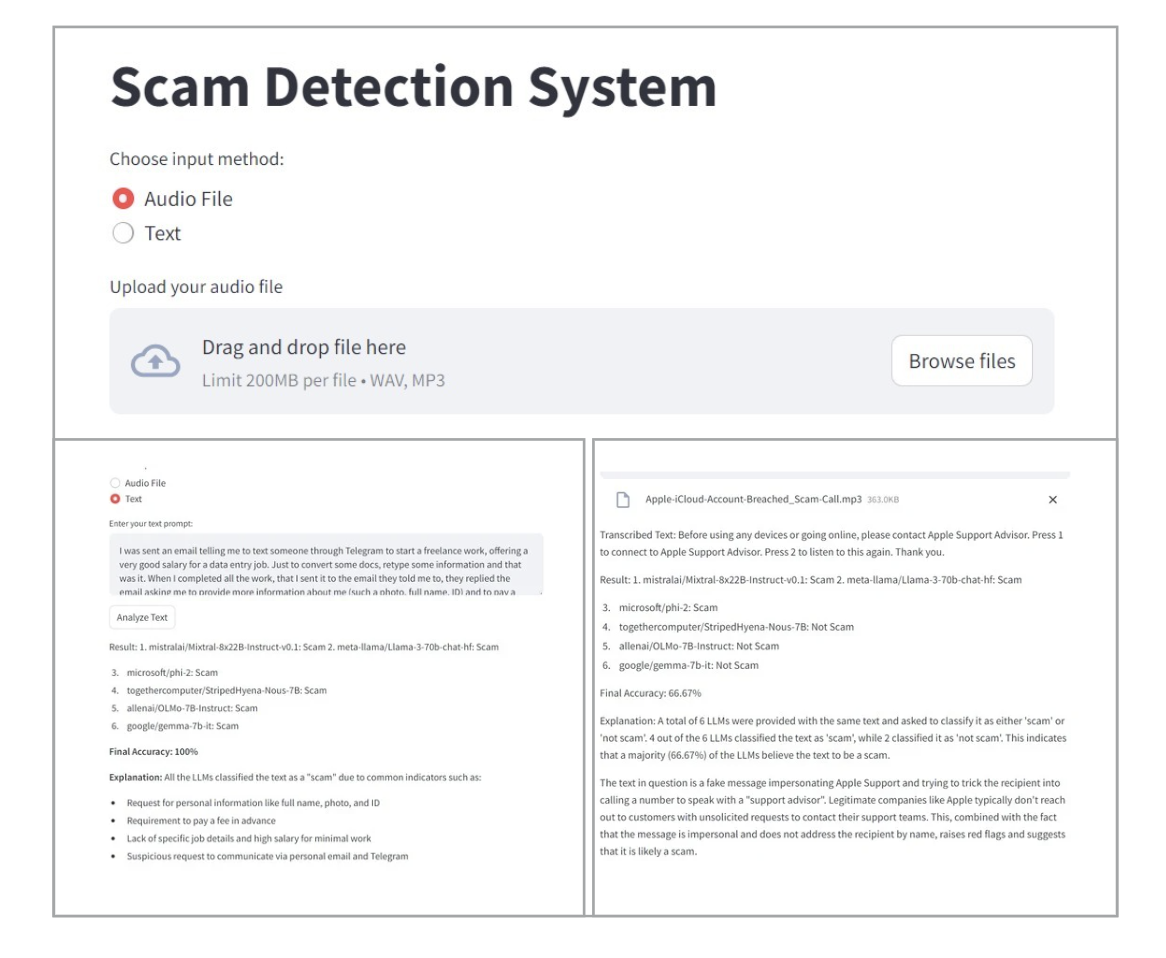
\includegraphics[width=0.8\textwidth]{demo.png} 
    \caption{Application Demonstartion: Top Image: Main landing page,
    Bottom Left and right: Scam detection using text and audio input respectively }
    \label{fig:demo}
\end{figure*}

\section{Contribution}
All members worked on conceptual system design. Areeb and Sameer worked on LLMs integration in Streamlit. Ubaid worked on user interface. Naveed handled the maintenance of Github repository, integrated Whisper module with streamlit and assissted Ubaid in UI integration. Amna authored the report, refined the GPT prompts and assisted Areeb with Gemini prompts. 

\begin{thebibliography}{}

\bibitem[\protect\citename{Radford et al.}2022]{radford2022robust}
Alec Radford, Jong Wook Kim, Tao Xu, Greg Brockman, Christine McLeavey, and Ilya Sutskever.
\newblock 2022.
\newblock {\em Robust Speech Recognition via Large-Scale Weak Supervision}.
\newblock arXiv preprint arXiv:2212.04356.

\bibitem[\protect\citename{Koide et al.}2024]{koide2024chatspamdetector}Takashi Koide, et al.
\newblock 2024.
\newblock {\em ChatSpamDetector: Leveraging Large Language Models for Effective Phishing Email Detection}.
\newblock arXiv preprint arXiv:2402.18093.

\bibitem[\protect\citename{Patel et al.}2024]{patel2024largelanguagemodels}
Het Patel, Umair Rehman, and Farkhund Iqbal.
\newblock 2024.
\newblock {\em Large Language Models Spot Phishing Emails with Surprising Accuracy: A Comparative Analysis of Performance}.
\newblock arXiv preprint arXiv:2404.15485.


\end{thebibliography}

\end{document}